\documentclass[12pt,a4paper]{article}

% ---- Core packages ----
\usepackage[margin=2.5cm, headheight=15pt]{geometry}
\usepackage[T1]{fontenc}
\usepackage[utf8]{inputenc}
\usepackage{lmodern}
\usepackage{microtype}
\usepackage{graphicx}
\usepackage{booktabs}
\usepackage{tabularx}
\usepackage{array}
\usepackage{multirow}
\usepackage{xcolor}
\usepackage{hyperref}
\usepackage{listings}
\usepackage{enumitem}
\usepackage{titlesec}
\usepackage{fancyhdr}
\usepackage{float}
\usepackage{caption}
\usepackage{subcaption}
\usepackage{mdframed}
\usepackage{amsmath}
\usepackage{tikz}
\usetikzlibrary{positioning,shapes.geometric,arrows.meta,fit,backgrounds,calc,shadows}

% ---- Colors ----
\definecolor{secblue}{RGB}{30,100,180}
\definecolor{subsecblue}{RGB}{52,130,200}
\definecolor{figcap}{RGB}{41,128,185}
\definecolor{termbg}{RGB}{22,22,22}
\definecolor{termfg}{RGB}{220,220,220}
\definecolor{termyellow}{RGB}{241,196,15}
\definecolor{termgreen}{RGB}{80,200,120}
\definecolor{nodehead}{RGB}{74,85,104}
\definecolor{nodeworker}{RGB}{56,142,102}
\definecolor{successcol}{RGB}{39,174,96}
\definecolor{plannedcol}{RGB}{230,126,34}
\definecolor{lightblue}{RGB}{210,228,245}
\definecolor{slidetitle}{RGB}{180,198,230}

% ---- Hyperref ----
\hypersetup{
  colorlinks=true, linkcolor=secblue, urlcolor=secblue,
  pdftitle={Ray Cluster Management — Workshop Progress Report},
  pdfauthor={Jahangir}
}

% ---- Headers / Footers ----
\pagestyle{fancy}\fancyhf{}
\fancyhead[L]{\small Progress Report}
\fancyhead[R]{\small Ray Cluster Management Workshop}
\fancyfoot[C]{\thepage}
\renewcommand{\headrulewidth}{0.4pt}

% ---- Section headings ----
\titleformat{\section}{\large\bfseries\color{secblue}}{\thesection}{0.6em}{}
\titleformat{\subsection}{\normalsize\bfseries\color{subsecblue}}{\thesubsection}{0.5em}{}
\titleformat{\subsubsection}{\normalsize\itshape\color{subsecblue}}{\thesubsubsection}{0.5em}{}

% ---- Caption style (match reference: coloured italic label) ----
\captionsetup{labelfont={bf,color=figcap}, textfont={it}, labelsep=period}

% ---- Listings (terminal style) ----
\lstdefinestyle{terminal}{
  backgroundcolor=\color{termbg},
  basicstyle=\footnotesize\ttfamily\color{termfg},
  breaklines=true, frame=single, rulecolor=\color{gray!40},
  numbers=none, xleftmargin=4pt, xrightmargin=4pt,
  aboveskip=4pt, belowskip=4pt,
  keywordstyle=\color{termyellow},
  stringstyle=\color{termgreen},
}
\lstdefinestyle{pycode}{
  backgroundcolor=\color{gray!8},
  basicstyle=\footnotesize\ttfamily,
  breaklines=true, frame=single, rulecolor=\color{gray!30},
  numbers=none, xleftmargin=4pt, xrightmargin=4pt,
  language=Python,
  keywordstyle=\color{secblue}\bfseries,
  commentstyle=\color{gray}\itshape,
  stringstyle=\color{successcol!80!black},
}
\lstset{style=terminal}

% ---- Slide-style framed figure box ----
\mdfdefinestyle{slidebox}{
  linecolor=gray!50, linewidth=0.8pt,
  innerleftmargin=10pt, innerrightmargin=10pt,
  innertopmargin=8pt, innerbottommargin=8pt,
  backgroundcolor=white
}

% Helper: slide title bar (matches presentation blue rounded box)
\newcommand{\slidetitlebar}[1]{%
  \begin{center}
    \fcolorbox{slidetitle!80!gray}{slidetitle!50}{%
      \parbox{0.72\linewidth}{\centering\bfseries #1}%
    }
  \end{center}
  \smallskip
}

% ---- TikZ node styles ----
\tikzset{
  headnode/.style={draw=nodehead, fill=nodehead, text=white, rounded corners=3pt,
                   minimum width=3.8cm, minimum height=0.55cm, font=\footnotesize\bfseries, align=center},
  workernode/.style={draw=nodeworker!80!black, fill=nodeworker, text=white, rounded corners=3pt,
                     minimum width=2.7cm, minimum height=0.55cm, font=\footnotesize\bfseries, align=center},
  svcbox/.style={draw=lightblue!80!gray, fill=lightblue, rounded corners=2pt,
                 minimum width=3.2cm, minimum height=0.48cm, font=\scriptsize, align=center},
  raylayer/.style={draw=gray!60, minimum width=5.6cm, minimum height=0.75cm,
                   font=\small, align=center},
  flowbox/.style={draw=secblue!70, fill=secblue!10, rounded corners=4pt,
                  minimum width=2.6cm, minimum height=0.7cm, font=\footnotesize, align=center},
  arr/.style={-Latex, thick, gray!70},
  barnode/.style={draw=none, minimum height=0.5cm, font=\footnotesize\bfseries, align=left}
}

% ============================================================
\begin{document}

% ---- Title block (matches reference — no separate page) ----
\begin{center}
  {\LARGE\bfseries\color{secblue} Ray Cluster Management Workshop}\\[0.5em]
  {\large Progress Report --- Workshop Delivered and Work Completed}\\[1em]
  {\normalsize Jahangir}\\[0.3em]
  {\normalsize 19 June 2026}
\end{center}

\vspace{0.8em}

\begin{abstract}
This report summarises the Ray Cluster Management Workshop delivered on
19~June~2026 on a live eight-node GPU cluster (268~CPUs, 8~GPUs,
192~GB~VRAM total). The session was structured as four progressive
parts --- Foundations, Deployment, Using the Cluster, and Hands-On
Examples --- and covered the complete workflow from bare-metal cluster
setup through distributed PyTorch training of a Llama~3.1-8B model and
multi-node LLM inference serving via vLLM and Ray. The report describes
what was demonstrated, includes diagrams reproduced from the presentation
slides, and records the key performance results obtained on the live
cluster during the session.
\end{abstract}

\tableofcontents
\newpage

% ============================================================
\section{Executive Summary}

The workshop guided participants through deploying and operating a
production Ray cluster, progressing from first-principles understanding
of the Ray framework to hands-on distributed training of large language
models and multi-node inference serving. All demonstrations ran on live
hardware visible to the room.

Two complementary bodies of work were presented.

\begin{enumerate}
\item \textbf{A deployed cluster and training pipeline.} A physical
eight-node cluster --- five RTX~4500~Ada and three RTX~3090 GPUs, all
connected over a 1\,Gb Ethernet switch --- was set up from scratch using
the Manual CLI method and used to run distributed PyTorch training from
ResNet-152 DDP through FSDP-sharded Llama~3.1-8B. All experiments were
tracked in MLflow with metrics, parameters, and model checkpoints stored
on NFS shared storage.

\item \textbf{A structured workshop curriculum.} The accompanying
presentation (38 slides, four parts) explained Ray's architecture, the
three deployment strategies, cluster usage patterns, and the vLLM
multi-node serving pipeline, framed around live results from the cluster.
\end{enumerate}

The headline performance result, demonstrated live, was a
\textbf{9.2$\times$ speedup} on a 300-task matrix-multiplication
benchmark: 156\,s on a single machine versus 17\,s on the eight-node
cluster. The Llama~3.1-8B FSDP training job completed with status
\textbf{SUCCEEDED} in \textbf{2\,h\,49\,min} across all eight GPUs.

% ============================================================
\section{Cluster Infrastructure}

\subsection{Hardware}

The physical cluster comprises eight heterogeneous GPU nodes on a shared
1\,Gb LAN. Table~\ref{tab:nodes} lists each node and its role.

\begin{table}[H]
\centering
\caption{Physical cluster nodes and assigned roles.}
\label{tab:nodes}
\begin{tabular}{lllll}
\toprule
\textbf{Node} & \textbf{IP} & \textbf{GPU} & \textbf{VRAM} & \textbf{Role} \\
\midrule
pc3-4500 & 192.168.3.73 & RTX 4500 Ada & 24\,GB & Head + Worker \\
pc1-4500 & 192.168.3.71 & RTX 4500 Ada & 24\,GB & Worker 1 \\
pc2-4500 & 192.168.3.72 & RTX 4500 Ada & 24\,GB & Worker 2 \\
pc4-4500 & 192.168.3.74 & RTX 4500 Ada & 24\,GB & Worker 3 \\
pc5-4500 & 192.168.3.75 & RTX 4500 Ada & 24\,GB & Worker 4 \\
pc6-3090 & 192.168.3.76 & RTX 3090     & 24\,GB & Worker 5 \\
pc7-3090 & 192.168.3.77 & RTX 3090     & 24\,GB & Worker 6 \\
pc8-3090 & 192.168.3.78 & RTX 3090     & 24\,GB & Worker 7 \\
\midrule
\multicolumn{2}{l}{\textbf{Total}} & 8 GPUs & 192\,GB & 268 CPUs \\
\bottomrule
\end{tabular}
\end{table}

Figure~\ref{fig:clusterarch} reproduces the cluster architecture diagram
from the presentation, showing the services hosted on the head node and
the seven task-execution workers.

\begin{figure}[H]
\begin{mdframed}[style=slidebox]
\slidetitlebar{Cluster Architecture}
\begin{center}
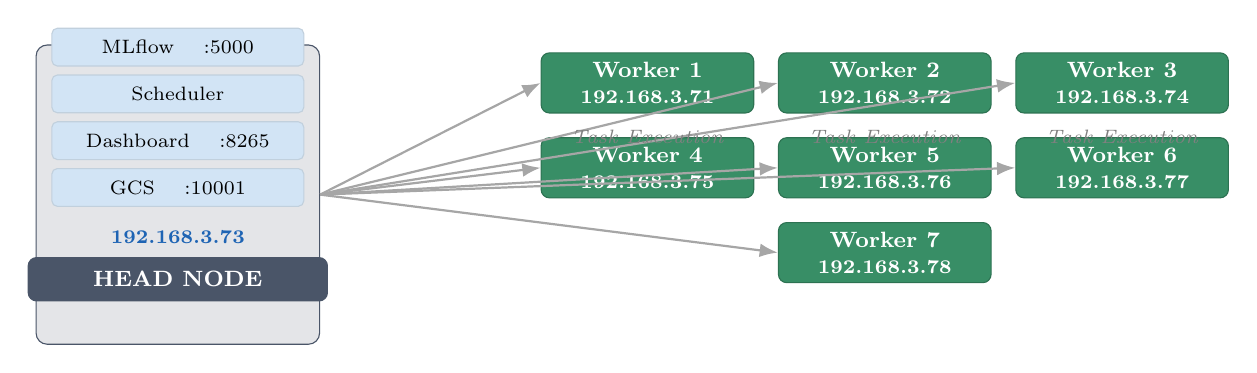
\begin{tikzpicture}[node distance=0.38cm and 0.3cm]
  % Head node outer box
  \node[draw=nodehead, fill=nodehead!15, rounded corners=4pt,
        minimum width=3.6cm, minimum height=3.8cm] (headbox) at (0,0) {};
  \node[headnode, above=0.55cm of headbox.south] (headlabel) {HEAD NODE};
  \node[font=\scriptsize\bfseries\color{secblue}, above=0.05cm of headlabel]
        (headip) {192.168.3.73};
  \node[svcbox, above=0.18cm of headip] (gcs) {GCS \quad :10001};
  \node[svcbox, above=0.1cm of gcs]    (dash) {Dashboard \quad :8265};
  \node[svcbox, above=0.1cm of dash]   (sched) {Scheduler};
  \node[svcbox, above=0.1cm of sched]  (mlf)  {MLflow \quad :5000};

  % Worker grid
  \node[workernode, right=2.8cm of headbox.north east, anchor=north west,
        yshift=-0.1cm] (w1) {Worker 1\\{\scriptsize 192.168.3.71}};
  \node[workernode, right=0.3cm of w1] (w2) {Worker 2\\{\scriptsize 192.168.3.72}};
  \node[workernode, right=0.3cm of w2] (w3) {Worker 3\\{\scriptsize 192.168.3.74}};
  \node[workernode, below=0.3cm of w1] (w4) {Worker 4\\{\scriptsize 192.168.3.75}};
  \node[workernode, below=0.3cm of w2] (w5) {Worker 5\\{\scriptsize 192.168.3.76}};
  \node[workernode, below=0.3cm of w3] (w6) {Worker 6\\{\scriptsize 192.168.3.77}};
  \node[workernode, below=0.3cm of w5] (w7) {Worker 7\\{\scriptsize 192.168.3.78}};

  % Arrows from head to workers
  \foreach \w in {w1,w2,w3,w4,w5,w6,w7}{
    \draw[arr] (headbox.east) -- (\w.west);
  }

  % Task execution labels
  \node[font=\scriptsize\itshape\color{gray},
        below=0.08cm of w1] {\scriptsize Task Execution};
  \node[font=\scriptsize\itshape\color{gray},
        below=0.08cm of w2] {\scriptsize Task Execution};
  \node[font=\scriptsize\itshape\color{gray},
        below=0.08cm of w3] {\scriptsize Task Execution};
\end{tikzpicture}
\end{center}
\end{mdframed}
\caption{Cluster architecture as presented: the head node (192.168.3.73) hosts the
  Global Control Store, Dashboard, Scheduler, and MLflow server; the seven worker
  nodes execute distributed tasks.}
\label{fig:clusterarch}
\end{figure}

\subsection{Network Topology}

All nodes connect through a single 1\,Gb Ethernet switch. The network
speed was verified on each node with \texttt{ethtool}, confirming
\texttt{Speed: 1000\,Mb/s} and \texttt{Link detected: yes} on every
interface. Figure~\ref{fig:network} reproduces the topology diagram
from the presentation.

\begin{figure}[H]
\begin{mdframed}[style=slidebox]
\slidetitlebar{Physical Cluster Connection Diagram}
\begin{center}
{\footnotesize\textsc{Network Topology: 1\,G Data Plane}}
\vspace{0.4em}

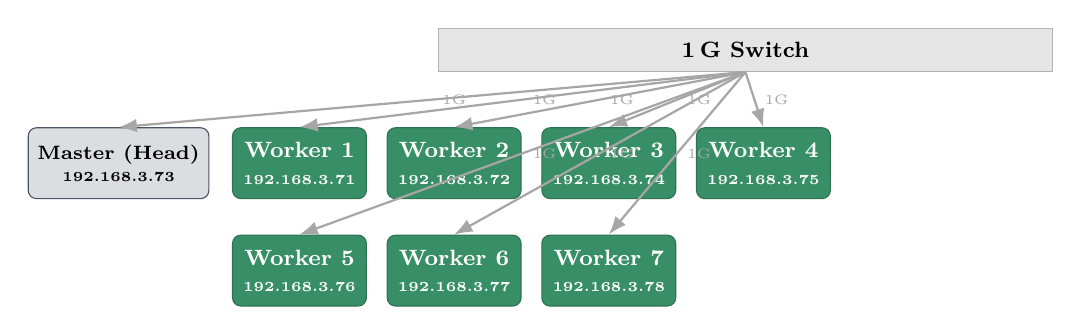
\begin{tikzpicture}[node distance=0.5cm]
  % Switch
  \node[draw=gray!60, fill=gray!20, minimum width=7.8cm, minimum height=0.55cm,
        font=\footnotesize\bfseries] (sw) {1\,G Switch};

  % Top row: Master + Workers 1-4
  \node[draw=nodehead, fill=nodehead!20, rounded corners=3pt,
        minimum width=1.8cm, minimum height=0.9cm, font=\scriptsize\bfseries,
        align=center, below left=0.7cm and 2.9cm of sw] (master)
        {Master (Head)\\{\tiny 192.168.3.73}};

  \node[workernode, minimum width=1.7cm, minimum height=0.9cm, align=center,
        below left=0.7cm and 0.9cm of sw] (n1)
        {Worker 1\\{\tiny 192.168.3.71}};
  \node[workernode, minimum width=1.7cm, minimum height=0.9cm, align=center,
        right=0.25cm of n1] (n2)
        {Worker 2\\{\tiny 192.168.3.72}};
  \node[workernode, minimum width=1.7cm, minimum height=0.9cm, align=center,
        right=0.25cm of n2] (n3)
        {Worker 3\\{\tiny 192.168.3.74}};
  \node[workernode, minimum width=1.7cm, minimum height=0.9cm, align=center,
        right=0.25cm of n3, align=center] (n4)
        {Worker 4\\{\tiny 192.168.3.75}};

  % Bottom row: Workers 5-7
  \node[workernode, minimum width=1.7cm, minimum height=0.9cm, align=center,
        below=0.45cm of n1] (n5)
        {Worker 5\\{\tiny 192.168.3.76}};
  \node[workernode, minimum width=1.7cm, minimum height=0.9cm, align=center,
        right=0.25cm of n5] (n6)
        {Worker 6\\{\tiny 192.168.3.77}};
  \node[workernode, minimum width=1.7cm, minimum height=0.9cm, align=center,
        right=0.25cm of n6] (n7)
        {Worker 7\\{\tiny 192.168.3.78}};

  % 1G labels on links
  \foreach \n in {master,n1,n2,n3,n4}{
    \draw[arr] (sw.south) -- (\n.north)
      node[midway, right, font=\tiny\color{gray}] {1G};
  }
  \foreach \n in {n5,n6,n7}{
    \draw[arr] (sw.south) -- (\n.north)
      node[midway, right, font=\tiny\color{gray}] {1G};
  }
\end{tikzpicture}
\end{center}
\end{mdframed}
\caption{Physical network topology: all eight nodes connect to a single 1\,Gb
  Ethernet switch. Verified link speed: 1000\,Mb/s on every node.}
\label{fig:network}
\end{figure}

% ============================================================
\section{Workshop Structure}

The workshop was delivered as four sequential parts, each building on
the previous. Table~\ref{tab:outline} shows the full outline.

\begin{table}[H]
\centering
\caption{Four-part workshop outline.}
\label{tab:outline}
\begin{tabular}{lll}
\toprule
\textbf{Part} & \textbf{Title} & \textbf{Topics covered} \\
\midrule
1 & Foundations     & What is Ray?, Ecosystem, Physical Cluster, Network \\
2 & Deployment      & Methods, Installation, Dashboard, MLflow, NFS \\
3 & Using the Cluster & Connection, Job submission, Matrix mult., Train, vLLM \\
4 & Hands-On Examples & Ray Core, Ray Train, vLLM on 8 GPUs \\
\bottomrule
\end{tabular}
\end{table}

% ============================================================
\section{Part 1 --- Foundations}

\subsection{What is Ray?}

Ray is an open-source distributed computing framework that scales Python
and AI workloads from a single machine to a cluster of thousands of
nodes. The core value proposition is that the programmer writes ordinary
Python; Ray's scheduler, object store, and fault-tolerant runtime handle
the distribution transparently. The same code runs on a laptop or a
1\,000-node cluster, and native GPU resource tracking means no manual
device placement across heterogeneous nodes.

\subsection{The Ray Ecosystem}

Figure~\ref{fig:ecosystem} reproduces the ecosystem architecture from
the presentation, showing the layered stack from compute infrastructure
through Ray~Core and Ray's high-level libraries, and the position of
vLLM as an optional execution backend that sits on top of the same
physical compute layer.

\begin{figure}[H]
\begin{mdframed}[style=slidebox]
\slidetitlebar{The Ray Ecosystem}
\begin{center}
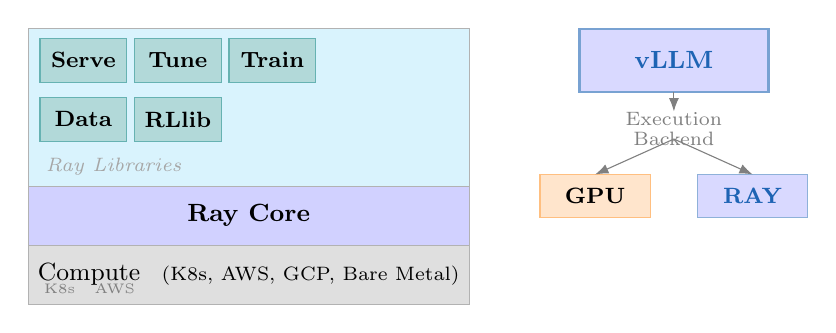
\begin{tikzpicture}
  %% Left: stacked layers
  % Compute
  \fill[gray!25] (0,0) rectangle (5.6,0.75);
  \draw[gray!60] (0,0) rectangle (5.6,0.75);
  \node[font=\small] at (2.8,0.375) {Compute \enspace {\scriptsize(K8s, AWS, GCP, Bare Metal)}};
  % Small cloud/k8s icons hint
  \node[font=\tiny\color{gray}] at (0.4,0.2) {K8s};
  \node[font=\tiny\color{gray}] at (1.1,0.2) {AWS};

  % Ray Core
  \fill[blue!18] (0,0.75) rectangle (5.6,1.5);
  \draw[gray!60] (0,0.75) rectangle (5.6,1.5);
  \node[font=\small\bfseries] at (2.8,1.125) {Ray Core};

  % Ray Libraries outer box
  \fill[cyan!15] (0,1.5) rectangle (5.6,3.5);
  \draw[gray!60] (0,1.5) rectangle (5.6,3.5);
  \node[font=\scriptsize\itshape, anchor=south west, color=gray!70] at (0.1,1.52)
       {Ray Libraries};

  % Library tiles
  \foreach \lbl/\x/\y in {
      Serve/0.7/3.1, Tune/1.9/3.1, Train/3.1/3.1,
      Data/0.7/2.35, RLlib/1.9/2.35}{
    \fill[teal!30] (\x-0.55,\y-0.28) rectangle (\x+0.55,\y+0.28);
    \draw[teal!60] (\x-0.55,\y-0.28) rectangle (\x+0.55,\y+0.28);
    \node[font=\footnotesize\bfseries] at (\x,\y) {\lbl};
  }

  %% Right: vLLM execution backend
  \fill[blue!15] (7.0,2.7) rectangle (9.4,3.5);
  \draw[secblue!60,thick] (7.0,2.7) rectangle (9.4,3.5);
  \node[font=\small\bfseries\color{secblue}] at (8.2,3.1) {vLLM};

  \node[font=\scriptsize, color=gray] at (8.2,2.35) {Execution};
  \node[font=\scriptsize, color=gray] at (8.2,2.1)  {Backend};
  \draw[-Latex,gray] (8.2,2.7) -- (8.2,2.45);

  % GPU box
  \fill[orange!20] (6.5,1.1) rectangle (7.9,1.65);
  \draw[orange!50] (6.5,1.1) rectangle (7.9,1.65);
  \node[font=\footnotesize\bfseries] at (7.2,1.375) {GPU};

  % RAY box
  \fill[blue!15] (8.5,1.1) rectangle (9.9,1.65);
  \draw[secblue!50] (8.5,1.1) rectangle (9.9,1.65);
  \node[font=\footnotesize\bfseries\color{secblue}] at (9.2,1.375) {RAY};

  \draw[-Latex,gray] (8.2,2.1) -- (7.2,1.65);
  \draw[-Latex,gray] (8.2,2.1) -- (9.2,1.65);
\end{tikzpicture}
\end{center}
\end{mdframed}
\caption{The Ray ecosystem: compute infrastructure underpins Ray~Core, which in turn
  supports six high-level libraries. vLLM uses Ray as its distributed executor backend,
  sitting on the same compute layer.}
\label{fig:ecosystem}
\end{figure}

Table~\ref{tab:ecosystem} summarises each library's role as introduced in the
presentation.

\begin{table}[H]
\centering
\caption{Ray library ecosystem.}
\label{tab:ecosystem}
\begin{tabularx}{\textwidth}{lX}
\toprule
\textbf{Library} & \textbf{Role} \\
\midrule
Ray Core  & Low-level \texttt{@ray.remote} task and actor API --- the foundation for all higher libraries \\
Ray Train & Distributed training for PyTorch, TensorFlow, XGBoost, HuggingFace; supports DDP and FSDP \\
Ray Tune  & Hyperparameter optimisation with pluggable backends (Optuna, ASHA, PBT); thousands of parallel trials \\
Ray Serve & Online model serving with autoscaling; any Python function as an HTTP endpoint \\
Ray Data  & Distributed data loading and preprocessing; chains natively into Train/Tune pipelines \\
Ray RLlib & Reinforcement learning at scale (PPO, SAC, etc.); automatic rollout worker distribution \\
\bottomrule
\end{tabularx}
\end{table}

% ============================================================
\section{Part 2 --- Deployment}

\subsection{Deployment methods}

Three deployment strategies were introduced and compared. The workshop
focused entirely on the \textbf{Manual CLI} method, which is most
transparent for learning and is appropriate for fixed bare-metal
clusters.

\begin{table}[H]
\centering
\caption{Deployment method comparison as shown in the presentation.}
\label{tab:deploy}
\begin{tabular}{lllll}
\toprule
\textbf{Method} & \textbf{Environment} & \textbf{Complexity} & \textbf{Auto-scale} & \textbf{Best For} \\
\midrule
Manual CLI     & Bare metal / VMs & Low    & No     & Learning, fixed clusters \\
Docker Compose & Single host      & Medium & Manual & Dev, demos, CI/CD \\
KubeRay        & Kubernetes       & High   & Yes    & Production, cloud-native \\
\bottomrule
\end{tabular}
\end{table}

\subsection{Installation and cluster startup}

Ray was installed identically on every node using a Conda environment:

\begin{lstlisting}[style=terminal, caption={Installation --- same steps on all 8 nodes.}]
conda create -n ray-env python=3.12 -y
conda activate ray-env
pip install ray[default]
\end{lstlisting}

The head node was started with dashboard exposed on all interfaces,
then each worker joined by pointing at the head node's GCS address:

\begin{lstlisting}[style=terminal, caption={Head and worker startup.}]
# Head node (pc3-4500, 192.168.3.73)
ray start --head --port=6379 --dashboard-host=0.0.0.0

# Each worker node (repeat on Workers 1-7)
ray start --address='192.168.3.73:6379'
\end{lstlisting}

\subsection{Cluster verification}

After all workers joined, \texttt{ray status} from the head node
confirmed 8 active nodes and the full pool of cluster resources:

\begin{lstlisting}[style=terminal, caption={Live \texttt{ray status} output captured during the workshop.}]
======== Autoscaler status: 2026-06-10 15:20:04.317026 ========
Node status
Active:
  8 nodes  (no failures)

Resources
  Total Usage:
  0.0/268.0  CPU
  0.0/8.0    GPU
  0B/336.69GiB  memory
  0B/144.29GiB  object_store_memory
\end{lstlisting}

\subsection{Shared storage and MLflow}

NFS shared storage at \texttt{/mnt/cluster\_storage/} is mounted on
all eight nodes and must be active before any training job is submitted.
It holds three categories of data: MLflow run artifacts, training
checkpoints (saved at configurable step intervals), and shared datasets.

An MLflow tracking server runs on the head node at port 5000. Every
training script connects to it at startup so that metrics, parameters,
and model artifacts are centralised and visible across the team.

% ============================================================
\section{Part 3 --- Using the Cluster}

\subsection{Connecting from code}

The entry point for any cluster job is \texttt{ray.init(address=''auto'')}.
Combined with the \texttt{@ray.remote} decorator, this is the complete
API surface for launching distributed work:

\begin{lstlisting}[style=pycode, caption={Minimal cluster task: the pattern demonstrated in the workshop.}]
import ray

ray.init(address="auto")

@ray.remote
def matmul():
    A = np.full((4096, 4096), 0.5, dtype=np.float64)
    B = np.full((4096, 4096), 0.5, dtype=np.float64)
    return socket.gethostname(), float(np.matmul(A, B).sum())

futures = [matmul.remote() for _ in range(300)]
results = ray.get(futures)
ray.shutdown()
\end{lstlisting}

\subsection{Matrix multiplication --- single machine vs.\ cluster}

This benchmark was the first live demo of the session. Three hundred
$4096\!\times\!4096$ matrix multiplications were dispatched, first
serially on a single machine, then as \texttt{@ray.remote} tasks across
the cluster. Figure~\ref{fig:speedup} shows the result.

\begin{figure}[H]
\begin{mdframed}[style=slidebox]
\slidetitlebar{Matrix Multiplication: Single Node vs.\ Cluster}
\begin{center}
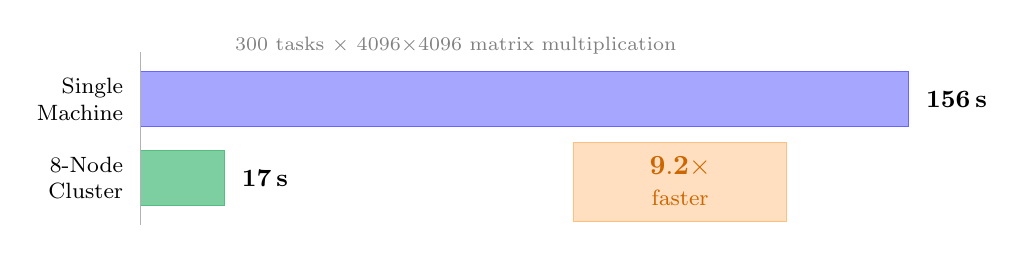
\begin{tikzpicture}
  % Axis labels
  \node[font=\footnotesize, anchor=east, align=right] at (-0.1,2.1) {Single\\Machine};
  \node[font=\footnotesize, anchor=east, align=right] at (-0.1,1.1) {8-Node\\Cluster};

  % Single machine bar (scaled: 156s -> 9.75cm)
  \fill[blue!35] (0,1.75) rectangle (9.75,2.45);
  \draw[blue!60] (0,1.75) rectangle (9.75,2.45);
  \node[font=\small\bfseries, anchor=west] at (9.85,2.1) {156\,s};

  % Cluster bar (scaled: 17s -> 1.06cm)
  \fill[successcol!60] (0,0.75) rectangle (1.06,1.45);
  \draw[successcol!80] (0,0.75) rectangle (1.06,1.45);
  \node[font=\small\bfseries, anchor=west] at (1.16,1.1) {17\,s};

  % Speedup badge
  \fill[orange!25] (5.5,0.55) rectangle (8.2,1.55);
  \draw[orange!50] (5.5,0.55) rectangle (8.2,1.55);
  \node[font=\bfseries\color{orange!80!black}] at (6.85,1.25)
        {$\mathbf{9.2\times}$};
  \node[font=\footnotesize\color{orange!80!black}] at (6.85,0.85)
        {faster};

  % Axis line
  \draw[gray!60] (0,0.5) -- (0,2.7);
  \node[font=\scriptsize\color{gray},above] at (4.0,2.55)
        {300 tasks $\times$ 4096$\times$4096 matrix multiplication};
\end{tikzpicture}

\medskip
{\footnotesize
Task distribution across the 8 nodes (Ray automatic scheduling):}
\smallskip

\begin{tabular}{llll}
pc8-3090 & 54 tasks & pc7-3090 & 36 tasks \\
pc3-4500 & 39 tasks & pc4-4500 & 32 tasks \\
pc6-3090 & 39 tasks & pc5-4500 & 32 tasks \\
pc2-4500 & 36 tasks & pc1-4500 & 32 tasks \\
\end{tabular}
\end{center}
\end{mdframed}
\caption{Live benchmark result: 300 matrix multiplications on a single machine took
  156\,s; the same workload dispatched as Ray tasks across the 8-node cluster completed
  in 17\,s --- a 9.2$\times$ speedup. Task distribution was determined automatically
  by the Ray scheduler.}
\label{fig:speedup}
\end{figure}

\subsection{Ray Train --- distributed PyTorch}

Nine training scripts of increasing complexity were presented, split
into two categories: vision/ViT models (ResNet and ViT families, scripts
1--5) and large language models (GPT-2 and Llama families, scripts
6--9). Table~\ref{tab:train} lists the full set.

\begin{table}[H]
\centering
\caption{Ray Train example scripts demonstrated during the workshop.}
\label{tab:train}
\begin{tabularx}{\textwidth}{clXl}
\toprule
\textbf{\#} & \textbf{Model} & \textbf{Training strategy} & \textbf{Category} \\
\midrule
1 & ResNet-152  & Single-GPU baseline                & \multirow{5}{*}{Vision / ViT} \\
2 & ResNet-152  & DDP across all 8 GPUs              & \\
3 & ResNet-18   & DDP + TensorBoard profiler          & \\
4 & ViT-Small   & FSDP2                              & \\
5 & ViT-H/14    & FSDP2 (large model)                & \\
\midrule
6 & GPT-2       & FSDP2 on WikiText-2                & \multirow{4}{*}{LLMs} \\
7 & GPT-2       & FSDP2 on TinyStories               & \\
8 & GPT-2       & FSDP2 + MLflow tracking            & \\
9 & Llama 3.1-8B & FSDP2 across all 8 GPUs           & \\
\bottomrule
\end{tabularx}
\end{table}

The Llama~3.1-8B FSDP training job (script~9) was the centrepiece of
Part~3. All eight workers were confirmed active in the startup log:

\begin{lstlisting}[style=terminal, caption={Ray Train log confirming 8-GPU FSDP worker group.}]
[TrainController] Requesting resources: {'GPU': 1} * 8
[TrainController] Starting worker group of size 8:
  ip=192.168.3.78  world_rank=0  node_rank=0
  ip=192.168.3.76  world_rank=1  node_rank=1
  ip=192.168.3.77  world_rank=2  node_rank=2
  ip=192.168.3.73  world_rank=3  node_rank=3
  ip=192.168.3.72  world_rank=4  node_rank=4
  ip=192.168.3.74  world_rank=5  node_rank=5
  ip=192.168.3.71  world_rank=6  node_rank=6
  ip=192.168.3.75  world_rank=7  node_rank=7
[RayTrainWorker] FSDP2 sharding complete.
[MLflow] Run: http://192.168.3.73:5000/#/experiments/5/runs/47b5d38fa77740c9b24...
\end{lstlisting}

The Ray Dashboard showed the job completing with status
\textbf{SUCCEEDED} after \textbf{2\,h\,49\,min}, with all 10\,000 Ray
tasks finishing without failures.

\subsection{vLLM with Ray --- multi-node LLM inference}

Llama~3.1-8B was deployed as a live inference server spread across all
eight GPU nodes using vLLM's pipeline-parallelism with Ray as the
distributed executor. Figure~\ref{fig:vllmpipeline} shows the serving
pipeline.

\begin{figure}[H]
\begin{mdframed}[style=slidebox]
\slidetitlebar{vLLM with Ray --- Serving Architecture}
\begin{center}
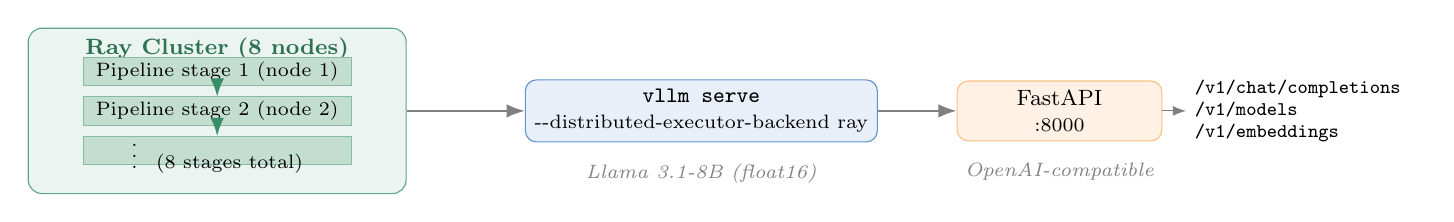
\begin{tikzpicture}[node distance=0.5cm and 0.6cm]
  % Ray cluster box
  \node[draw=nodeworker!80, fill=nodeworker!10, rounded corners=5pt,
        minimum width=4.8cm, minimum height=2.1cm] (raycluster) {};
  \node[font=\footnotesize\bfseries\color{nodeworker!80!black},
        anchor=north] at (raycluster.north) {Ray Cluster (8 nodes)};

  % Pipeline stages inside
  \foreach \i/\y in {0/0.5, 1/0, 2/-0.5}{
    \fill[nodeworker!30] (-1.7,\y-0.18) rectangle (1.7,\y+0.18);
    \draw[nodeworker!60] (-1.7,\y-0.18) rectangle (1.7,\y+0.18);
  }
  \node[font=\scriptsize] at (0, 0.5)  {Pipeline stage 1 (node 1)};
  \node[font=\scriptsize] at (0, 0.0)  {Pipeline stage 2 (node 2)};
  \node[font=\scriptsize] at (0,-0.5)  {$\vdots$ \enspace (8 stages total)};
  \draw[-Latex,thick,nodeworker] (0,0.32) -- (0,0.18);
  \draw[-Latex,thick,nodeworker] (0,-0.18) -- (0,-0.32);

  % vLLM serve command
  \node[flowbox, right=1.5cm of raycluster] (vllmserve)
        {\texttt{vllm serve}\\{\scriptsize{-{}-distributed-executor-backend ray}}};
  \draw[-Latex,gray,thick] (raycluster.east) -- (vllmserve.west);

  % FastAPI
  \node[flowbox, right=1.0cm of vllmserve, fill=orange!10, draw=orange!50]
       (api) {FastAPI\\{\scriptsize :8000}};
  \draw[-Latex,gray,thick] (vllmserve.east) -- (api.west);

  % Endpoints
  \node[font=\scriptsize, anchor=west, right=0.3cm of api,
        text width=2.8cm] (eps)
        {\texttt{/v1/chat/completions}\\
         \texttt{/v1/models}\\
         \texttt{/v1/embeddings}};
  \draw[-Latex,gray] (api.east) -- (eps.west);

  % Labels
  \node[font=\scriptsize\itshape\color{gray}, below=0.15cm of vllmserve]
       {Llama 3.1-8B (float16)};
  \node[font=\scriptsize\itshape\color{gray}, below=0.15cm of api]
       {OpenAI-compatible};
\end{tikzpicture}
\end{center}
\end{mdframed}
\caption{vLLM pipeline-parallel serving architecture demonstrated in the workshop.
  The model is sharded across 8 pipeline stages (one per GPU node); the Ray distributed
  executor coordinates token passing. The FastAPI server at port~8000 exposes an
  OpenAI-compatible HTTP API.}
\label{fig:vllmpipeline}
\end{figure}

The launch command issued on the head node:

\begin{lstlisting}[style=terminal, caption={vLLM multi-node launch command.}]
RAY_ADDRESS=192.168.3.73:6379 VLLM_PLUGINS="" \
vllm serve ~/projects/vllm-deployment/vllm/models/3.1-8b-instruct \
  --dtype float16 \
  --tensor-parallel-size 1 \
  --pipeline-parallel-size 7 \
  --distributed-executor-backend ray \
  --gpu-memory-utilization 0.4 \
  --max-model-len 1024 \
  --enforce-eager \
  --host 0.0.0.0 --port 8000
\end{lstlisting}

All eight nodes appeared as \textbf{ALIVE} in the Ray Dashboard with
active GRAM usage once the model had loaded. The \texttt{/v1/models}
endpoint confirmed \texttt{3.1-8b-instruct} as the active serving model.

\subsection{MLflow experiment tracking}

Every training run was tracked automatically. Figure~\ref{fig:mlflow}
summarises the MLflow pipeline used throughout Part~3.

\begin{figure}[H]
\begin{mdframed}[style=slidebox]
\slidetitlebar{MLflow: Experiment Tracking Pipeline}
\begin{center}
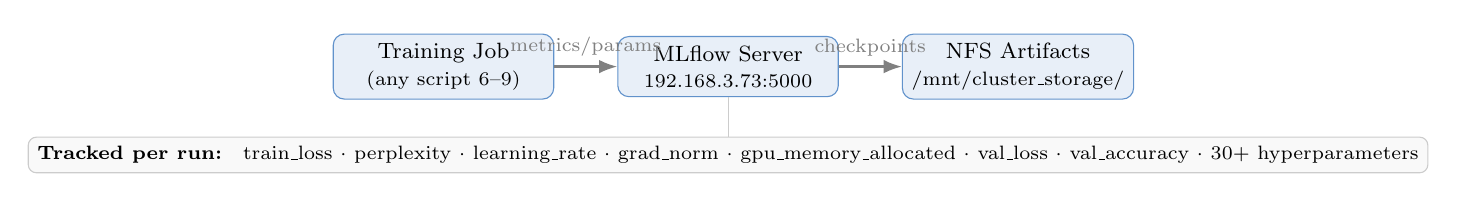
\begin{tikzpicture}[node distance=0.5cm and 0.8cm]
  \node[flowbox, minimum width=2.8cm] (job) {Training Job\\{\scriptsize(any script 6--9)}};
  \node[flowbox, minimum width=2.8cm, right=0.8cm of job] (mlf)
       {MLflow Server\\{\scriptsize 192.168.3.73:5000}};
  \node[flowbox, minimum width=2.8cm, right=0.8cm of mlf] (nfs)
       {NFS Artifacts\\{\scriptsize /mnt/cluster\_storage/}};

  \draw[-Latex,gray,thick] (job.east) -- (mlf.west)
        node[midway,above,font=\scriptsize] {metrics/params};
  \draw[-Latex,gray,thick] (mlf.east) -- (nfs.west)
        node[midway,above,font=\scriptsize] {checkpoints};

  % What's tracked
  \node[draw=gray!40, fill=gray!5, rounded corners=3pt,
        below=0.5cm of mlf, minimum width=9cm, font=\scriptsize,
        align=center] (tracked)
       {\textbf{Tracked per run:} \enspace
        train\_loss $\cdot$ perplexity $\cdot$ learning\_rate $\cdot$ grad\_norm $\cdot$
        gpu\_memory\_allocated $\cdot$ val\_loss $\cdot$ val\_accuracy
        $\cdot$ 30+ hyperparameters};
  \draw[gray!40] (mlf.south) -- (tracked.north);
\end{tikzpicture}
\end{center}
\end{mdframed}
\caption{MLflow experiment tracking pipeline used throughout the workshop. Every
  training script logs metrics and parameters to the head-node server; model checkpoints
  are written to NFS shared storage at configurable step intervals.}
\label{fig:mlflow}
\end{figure}

The live MLflow UI showed the Llama~3.1-8B run (named
\texttt{llama31\_8b\_fsdp}) with 12 tracked metrics and 30 recorded
parameters (model path, \texttt{num\_parameters}: 8\,030\,000\,000,
\texttt{num\_layers}: 32, \texttt{hidden\_size}: 4096, etc.).
Checkpoints were saved at 500-step intervals up to step~7500.

% ============================================================
\section{Part 4 --- Hands-On Examples}

\subsection{Examples status}

Table~\ref{tab:examples} records which examples were completed during
the workshop and which are planned for future sessions, exactly as shown
on the final status slide of the presentation.

\begin{table}[H]
\centering
\caption{Workshop examples --- completion status.}
\label{tab:examples}
\begin{tabular}{clll}
\toprule
\textbf{\#} & \textbf{Folder} & \textbf{Library} & \textbf{Status} \\
\midrule
1 & \texttt{1-ray-core/}       & Ray Core   &
    \textcolor{successcol}{\bfseries Completed} \\
2 & \texttt{2-ray-training/}   & Ray Train  &
    \textcolor{successcol}{\bfseries Completed} \\
3 & \texttt{3-RL-lib/}         & Ray RLlib  &
    \textcolor{plannedcol}{\bfseries Planned} \\
4 & \texttt{4-ray-serve(LLM)/} & Ray Serve  &
    \textcolor{plannedcol}{\bfseries Planned} \\
5 & \texttt{5-ray-tune/}       & Ray Tune   &
    \textcolor{plannedcol}{\bfseries Planned} \\
6 & \texttt{6.vllm/}           & vLLM + Ray &
    \textcolor{successcol}{\bfseries Completed} \\
\bottomrule
\end{tabular}
\end{table}

\subsection{Completed examples}

\textbf{Example 1 --- Ray Core.}
Two side-by-side scripts demonstrated the \texttt{@ray.remote} pattern:
square-root computations and matrix multiplications (the latter
producing the 9.2$\times$ speedup result above). Participants could
observe the dashboard distributing tasks in real time.

\textbf{Example 2 --- Ray Train.}
The training curriculum ran from a single-GPU ResNet-152 baseline
through DDP, FSDP2 on ViT-H/14, and finally FSDP2 on Llama~3.1-8B
across all eight cluster GPUs. The Llama job completed successfully in
2\,h\,49\,min. Three key implementation patterns were highlighted:
DDP via \texttt{prepare\_model()}/\texttt{prepare\_data\_loader()};
FSDP2 via \texttt{torch.distributed.fsdp.fully\_shard()} with a device
mesh and ``meta''-device model loading to avoid CPU OOM; and Ray Train
V2 enabled with \texttt{os.environ["RAY\_TRAIN\_V2\_ENABLED"]~=~"1"}.

\textbf{Example 6 --- vLLM on 8 GPUs.}
The end-to-end serving workflow was demonstrated: start cluster, launch
vLLM with Ray backend, verify GPU allocation in the Dashboard, and
query the OpenAI-compatible endpoint. The \texttt{/v1/chat/completions}
and \texttt{/v1/models} endpoints both responded correctly.

\subsection{Planned examples}

Three examples are scheduled for subsequent sessions:
\textit{Ray RLlib} (PPO reinforcement learning with automatic rollout
workers), \textit{Ray Serve} (autoscaling model serving with rolling
updates), and \textit{Ray Tune} (distributed hyperparameter search
using the Optuna backend).

% ============================================================
\section{Key Technical Points}

Several non-obvious implementation details were covered in the
workshop and are worth recording here for reference.

\begin{enumerate}

\item \textbf{Always declare resources on \texttt{@ray.remote}.}
Omitting \texttt{num\_gpus} and \texttt{num\_cpus} causes Ray to
default to 1~CPU and 0~GPUs per task, which can monopolise a single
node or leave all GPUs idle.

\item \textbf{Use \texttt{ray.put()} for large shared data.}
Passing a 10\,GB dataset directly into many task calls creates
duplicate copies in standard RAM. \texttt{ray.put()} stores the object
once in the zero-copy shared object store; workers receive a lightweight
\texttt{ObjectRef}.

\item \textbf{Submit via the Job CLI, not direct execution.}
\texttt{python my\_script.py} runs the driver locally and logs are only
visible in the terminal. \texttt{ray job submit \ldots} routes
everything through the Dashboard and makes \texttt{print()} output,
errors, and task graphs visible live in the browser.

\item \textbf{\texttt{GLOO\_SOCKET\_IFNAME} must be in the shell at
\texttt{ray start} time.}
A running Ray worker does not re-read \texttt{.bashrc}. Without this
variable, Gloo auto-detects Docker bridge interfaces (172.x.x.x range)
and the \texttt{connectFullMesh} handshake fails. After any change,
stop and restart the worker so it inherits the updated environment.

\item \textbf{FSDP large-model initialisation.}
Loading a model to CPU first and then sharding it with FSDP2 exhausts
RAM for 8B+ parameter models. The correct pattern is to create the
model on the \texttt{"meta"} device, apply \texttt{fully\_shard()},
then call \texttt{.to\_empty(device=device)} to allocate real memory
only after sharding is complete.

\item \textbf{Graceful shutdown.}
Always call \texttt{ray.shutdown()} at the end of driver scripts to
release GPU and CPU reservations back to the cluster pool.

\end{enumerate}

% ============================================================
\section{Conclusion}

The workshop successfully demonstrated the complete Ray cluster workflow
on live hardware. Three outcomes are immediately reproducible by
participants:

\begin{itemize}
\item A bare-metal eight-node Ray cluster can be assembled in under
fifteen minutes using the Manual CLI method and verified with
\texttt{ray status}.

\item Distributed PyTorch training --- up to and including an
8-billion-parameter FSDP-sharded language model --- can be submitted as
a single \texttt{ray job submit} command and tracked end-to-end in
MLflow and the Ray Dashboard.

\item A multi-node LLM inference server (Llama~3.1-8B, pipeline-parallel
across 8 GPUs) can be launched with a single \texttt{vllm serve}
command using \texttt{-{}-distributed-executor-backend ray}, and is
immediately accessible through an OpenAI-compatible HTTP API.
\end{itemize}

The three planned examples (Ray RLlib, Ray Serve, Ray Tune) will be
covered in a follow-up session, completing the full \texttt{examples/}
library in the workshop repository.

% ============================================================
\newpage
\section*{Workshop Photographs}
\addcontentsline{toc}{section}{Workshop Photographs}

The following pages contain photographs taken during the workshop
session on 19~June~2026.

\vspace{1.5em}

% ---- Photo grid ----
\begin{figure}[H]
\centering
\begin{subfigure}[t]{0.47\textwidth}
  \centering
  \fbox{\rule{0pt}{5.5cm}\hspace{\dimexpr\linewidth-2\fboxsep-2\fboxrule\relax}}
  \caption{Participants during the foundations section.}
\end{subfigure}
\hfill
\begin{subfigure}[t]{0.47\textwidth}
  \centering
  \fbox{\rule{0pt}{5.5cm}\hspace{\dimexpr\linewidth-2\fboxsep-2\fboxrule\relax}}
  \caption{Physical cluster hardware setup (8 nodes).}
\end{subfigure}
\caption{Workshop session --- Part 1: Foundations.}
\end{figure}

\begin{figure}[H]
\centering
\begin{subfigure}[t]{0.47\textwidth}
  \centering
  \fbox{\rule{0pt}{5.5cm}\hspace{\dimexpr\linewidth-2\fboxsep-2\fboxrule\relax}}
  \caption{Ray Dashboard showing all 8 nodes ALIVE.}
\end{subfigure}
\hfill
\begin{subfigure}[t]{0.47\textwidth}
  \centering
  \fbox{\rule{0pt}{5.5cm}\hspace{\dimexpr\linewidth-2\fboxsep-2\fboxrule\relax}}
  \caption{Matrix multiplication benchmark live result.}
\end{subfigure}
\caption{Workshop session --- Part 2 \& 3: Deployment and using the cluster.}
\end{figure}

\begin{figure}[H]
\centering
\fbox{\rule{0pt}{7.5cm}\hspace{\dimexpr\textwidth-2\fboxsep-2\fboxrule\relax}}
\caption{Llama 3.1-8B FSDP training job --- SUCCEEDED in 2\,h\,49\,min.}
\end{figure}

\begin{figure}[H]
\centering
\begin{subfigure}[t]{0.47\textwidth}
  \centering
  \fbox{\rule{0pt}{5.5cm}\hspace{\dimexpr\linewidth-2\fboxsep-2\fboxrule\relax}}
  \caption{vLLM + Ray: 8 GPUs serving Llama 3.1-8B.}
\end{subfigure}
\hfill
\begin{subfigure}[t]{0.47\textwidth}
  \centering
  \fbox{\rule{0pt}{5.5cm}\hspace{\dimexpr\linewidth-2\fboxsep-2\fboxrule\relax}}
  \caption{MLflow dashboard showing run metrics.}
\end{subfigure}
\caption{Workshop session --- Part 4: Hands-on vLLM demonstration.}
\end{figure}

\begin{figure}[H]
\centering
\begin{subfigure}[t]{0.47\textwidth}
  \centering
  \fbox{\rule{0pt}{5.5cm}\hspace{\dimexpr\linewidth-2\fboxsep-2\fboxrule\relax}}
  \caption{Q\&A and discussion.}
\end{subfigure}
\hfill
\begin{subfigure}[t]{0.47\textwidth}
  \centering
  \fbox{\rule{0pt}{5.5cm}\hspace{\dimexpr\linewidth-2\fboxsep-2\fboxrule\relax}}
  \caption{Group photograph.}
\end{subfigure}
\caption{Workshop close.}
\end{figure}

\vspace{1.5em}
\noindent\textit{To insert real photographs: replace each
\texttt{\textbackslash fbox\{\ldots\}} placeholder with
\texttt{\textbackslash includegraphics[width=\textbackslash linewidth]\{photos/filename.jpg\}}
and place the image files in a \texttt{photos/} folder next to this
\texttt{.tex} file.}

\end{document}
